\documentclass{ctexart}
\usepackage{PhysicalChemistryNote}

\begin{document}\pagestyle{plain}
\setcounter{footnote}{0}
\begin{center}
    \tbf{\Huge Chapter 7 化学反应动力学}
\end{center}\vspace{15pt}

\indent 想象一下:你小心翼翼地把面团塞进烤箱,等待它膨胀成蓬松的面包——但如果你打开烤箱的瞬间,%
面团就“唰”地变成了焦炭,或者干脆像被施了冰冻咒一样毫无变化,厨房大概会变成灾难现场吧?%
好在现实中,大多数化学反应都像一位慢性子的老管家,不慌不忙地按照自己的节奏工作.%
而化学动力学的使命,就是破解这位管家藏在围裙口袋里的“日程表”,%
搞清楚它为何有时慢吞吞,有时又像被踩了尾巴的猫一样蹿得飞快(比如嘭一声炸开的爆米花).\\
\indent 如果说热力学是化学界的“预言家”,只告诉你“面包最终会不会烤熟”,%
那么动力学就是那个举着秒表,贴着烤箱玻璃偷看的厨师.%
它不仅关心反应的终点,更执着于追踪过程中每一个微妙的时间刻度:为什么加一撮酵母能让面团在半小时内膨胀,而不是半年?%
为什么夏天牛奶变质的速度总让冰箱成为人类最伟大的发明之一?%
这些看似平常的现象背后,都藏着分子世界速度与激情的故事.\\
\indent 准备好了吗?带上你的好奇心(和计算器),我们要推开一扇新世界的大门了——%
在这里,时间不再是钟表的滴答声,而是分子们踢踏舞步的节奏,是能量起伏的山丘地图,更是人类掌控物质变换的终极秘籍.%
祝你好运!
\newpage\documentclass{ctexart}
\usepackage{PhysicalChemistryNote}

\begin{document}\pagestyle{plain}
\noindent\tbf{\LARGE 7A 化学反应的速率与速率方程}\vspace{15pt}\\
\indent 通常,化学反应的进行总是需要一定时间.有些反应总是进行得很快(例如炸药的爆炸),%
而有些反应的速度却相当让人着急(比如无催化剂下\ce{N2}与\ce{H2}反应生成\ce{NH3}).%
于是,我们希望用一种普适的量描述化学反应的速率,并且想办法求出速率与各个反应物的浓度的关联.\vspace{12pt}\\
\Section{7A.1 化学反应的速率}
\indent 我们先从速率如何定义入手学习描述反应速率的方法.
\begin{derivation}
    朴素地来看,如果单位时间内产生的产物(或消耗的反应物)越多,那么反应的速率应当越快.%
    不过,由于物质的量$n$是广度量,因此如果用它的变化衡量速率,就会出现与系统规模有关的问题.%
    因此,我们采用一定时间内某组分浓度的变化衡量反应速率是相对合理的.\\
    于是组分$i$的反应速率$v_i$就满足
    \[v_i=\dfrac{\di[i]}{\di t}=\dfrac{1}{V}\dfrac{\di n_i}{\di t}\]
    由于反应中各物质的计量数可能并不相同,因此用上面的方法得出的速率也各有差别.%
    回忆我们在热力学中消除这一影响的方法(见\tbf{5A.1.1}),我们可以用反应进度$\xi$代替$n_i$.这样就有
    \[v_i=\dfrac{1}{V}\dfrac{\di n_i}{\di t}=\nu_i\cdot\dfrac{1}{V}\dfrac{\di\xi}{\di t}\]
    这样,我们可以得到一个统一的速率$v=\dfrac{1}{V}\dfrac{\di\xi}{\di t}$.结合计量数$\nu_i$,就可以得出任意组分的反应速率$v_i$.
\end{derivation}
\begin{definition}[7A.1.1 化学反应的速率]
    (体积不变的均相系统中的)\tbf{化学反应的速率}$r$定义为反应进度$\xi$对时间$t$的变化率与系统体积$V$的比值,即
    \[v\xlongequal{\text{def}}\dfrac{1}{V}\dfrac{\di\xi}{\di t}\]
    对于非均相系统,常常
\end{definition}
从上面的推导中很容易得出速率与各物质产生/消耗的速率的关系.
\begin{theorem}[7A.1.2 反应速率与各物质生成/消耗速率的关系]
    
\end{theorem}
\end{document}
\newpage\documentclass{ctexart}
\usepackage{PhysicalChemistryNote}

\begin{document}\pagestyle{plain}
\noindent\tbf{\LARGE 7B 积分速率方程}\vspace{15pt}\\
\indent 如我们前面所述,速率方程事实上是一个关于物质浓度的微分方程,因而可以通过数学方法求解各物质浓度与时间的关系.%
在大多数情形下,这些微分方程都有精确的解析解\footnote{即有明确函数表达式的解.}.%
我们将在本节讨论常见速率方程及其解,并由此介绍其应用.\vspace{12pt}\\
\Section{7B.1 简单整数级反应}
\Part{零级反应}
\indent 我们从最简单的零级反应入手.零级反应的积分速率方程可以推导如下.
\begin{derivation}
    考虑反应\ce{A -> P},其速率方程为
    \[v=-\dfrac{\di\con{A}}{\di t}=k\]
    这是一个再简单不过的微分方程,我们移项可得
    \[\di\con{A}=-k\di t\]
    考虑起始时间为$0$,\ce{A}的起始浓度为$\con{A}_0$,对上式两边积分可得
    \[\con{A}-\con{A}_0=-kt\]
    即
    \[\con{A}=\con{A}_0-kt\]
    这表明$\con{A}$与时间$t$成一次函数关系.我们在下图中给出了\ce{A}的浓度随时间变化的图像.
    \begin{tightcenter}
        \documentclass{standalone}
\usepackage{PhysicalChemistryNote}
\begin{document}
\begin{tikzpicture}
    \draw[->] (0,0)--(6.5,0) node[right] {$t$};
    \draw[->] (0,0)--(0,4.5) node[above] {$\con{A}$};
    \draw[-] (0,4)--(6,0);
    \draw[-] (0,4)--(2,0);
    \fill (0,4) circle (1.5pt) node[left] {$\con{A}_0$};
    \fill (2,0) circle (1.5pt) node[below] {$t_1$};
    \fill (6,0) circle (1.5pt) node[below] {$t_2$};
    \node[right] at (1,2) {$k_1$};
    \node[right] at (3.1,2) {$k_2$};
\end{tikzpicture}
\end{document}
    \end{tightcenter}
    在\ce{A}反应完全后,反应便不再进行,保持$\con{A}=0$.
\end{derivation}
\end{document}
\newpage\documentclass{ctexart}
\usepackage{PhysicalChemistryNote}

\begin{document}\pagestyle{plain}
\noindent\tbf{\LARGE 7C 反应机理与速率方程的推导}\vspace{15pt}\\
\indent 化学反应在大多数情况下并不是一蹴而就的.例如葡萄糖\ce{C6H12O6}在你的身体里被氧化的过程:%
\ce{C6H12O6 + 6O2 -> 6CO2 + 6H2O}.显然,让一个\ce{C6H12O6}分子与六个\ce{O2}分子一步到位地生成%
六个\ce{CO2}分子与六个\ce{6H2O}分子是不大现实的,这需要所有\ce{O2}同时以合适的角度接近并发生反应,%
这一概率是非常低的.事实上我们知道,这一反应,乃至绝大多数反应都是通过数个步骤进行的,%
这些步骤构成了我们所讲的反应机理,并且也密切影响着反应的速率.\vspace{12pt}\\
\Section{7C.1 基元反应}
\Part{基元反应}
\indent 在前言中,我们说大部分反应都是通过数个步骤进行的.这些简单而基本的步骤就是我们所说的\tbf{基元反应}.
\begin{definition}[7C.1.1 基元反应]
    \tbf{基元反应}(或称\tbf{基本反应}),顾名思义,即最简单的化学反应步骤,是一个或多个化学物种直接作用,一步(即通过单一过渡态)转化为反应产物的过程.
\end{definition}
下面是几个常见的基元反应:
\begin{tightcenter}
    \ce{H. + Br2 -> HBr + Br.}\\
    \ce{CH3I + Cl- -> CH3Cl + I-}\\
    \ce{I2 -> 2I.}
\end{tightcenter}
可以看到,参与基元反应的物质并不一定是稳定的化合物,也可能是自由基等不稳定物种.并且,参与反应的分子数各不相同.
\begin{theorem}[7C.1.2 基元反应的分子数]
    基元反应的\tbf{分子数}是指参与基元反应的分子数.\\
    在\tbf{单分子反应}中,单个分子振动分解或发生重排.\\
    在\tbf{双分子反应}中,参与反应的两个分子以合适的方式碰撞,发生能量交换,键的生成和断裂等过程.\\
    一般而言,三分子反应已经很少见,而分子数大于等于四的基元反应几乎不存在.
\end{theorem}
基元反应,正由于其简单的特征,速率方程也十分简洁.
\begin{theorem}[7C.1.3 基元反应的速率方程]
    单分子基元反应对反应物为一级,其速率(以\ce{A -> P}为例)为$v=k\con{A}$.\\
    双分子基元反应对每个反应物都为一级(如果反应物相同就为二级),其速率(以\ce{A + B -> P}为例)为$v=k\con{A}\con{B}$,%
    或(以\ce{2A -> P}为例)为$v=k\con{A}^2$.
\end{theorem}
我们可以对上面的结论做定性的解释.%
在一定温度下,具有适合的能量的分子在总体中占的比例是一定的.因此,参与基元反应的物质的浓度越高,%
具有适合的能量的分子的浓度就越高,反应速率也就越快,并且对每个参与反应的分子的浓度都应当%
成正比例关系.\vspace{4pt}\\
\Part{微观可逆性原理和精细平衡原理}
\indent 直觉地来看,如果将描述物质运动的方程中的时间$t$和速度$v$替换成其负值,并不影响运动方程%
的成立.因此,运动的过程是可以通过恰好相反的方向进行的,而它们遵守相同的物理规律.这就是力学中的\tbf{时间反演对称性}%
\footnote{说得粗糙一些,这和时间倒流在某种程度上是一致的.如果你看过Christopher Nolan执导的电影《信条》,可能对这样的现象会有更为直观的认识.}.
\begin{hint}
    这一“直觉”事实上在经典力学和量子力学中都可以被证明,但由于涉及到一些复杂的物理知识,故在此并不给出.\\
    需要注意的是,由于我们在这里讨论的仅仅是单个或少数几个物体(即分子),因此尚不具有统计意义.%
    这要与热力学第二定律做区分.\\
    你可以简单地认为,力学肯定的是微观过程的可逆性,而统计物理学(以及热力学)肯定的是宏观过程的不可逆性,%
    两者讨论的范畴并不相同,因此也没有矛盾之处.
\end{hint}
以上我们从力学的角度讨论了时间反演对称性.它告诉我们,化学过程中反应的微粒服从力学方程(如基元反应中反应物微粒单次碰撞行为),%
则在正,逆反应过程中所经历的途径是相同的,逆过程要经历正过程的所有状态,就像一部电影从后往前倒过来放映,%
片中的一切动作是正常放映时动作的完全逆转;同时,在沿着反应坐标移动形成并最后解体的活化络合物的组成和结构在两个方向上是相同的,只不过动量的符号相反.%
由此,我们可以提出时间反演对称在化学动力学中的表述.
\begin{theorem}[7C.1.4 微观可逆性原理]
    如果一个正反应是基元反应,那么它的逆反应也是基元反应,且正逆反应具有相同的活化络合物(即中间体).
\end{theorem}
微观可逆性原理对假设反应厉程有明显的制约:它要求设想的反应机理中任一基元反应的逆反应不应是不可能的反应.%
如四乙基铅的气相分解反应:\ce{Pb(C2H5)4 -> Pb + 4C2H5.},逆反应是不可能发生的五分子反应,所以该反应不可能是基元反应.\\
\indent 到目前为止,我们似乎仍未考虑反应达到平衡的情形.此时,总体正反应和逆反应的速率相等,%
各物质的浓度不再随时间变化.那么具体到每个基元反应上又是何种情况呢?%
为此,人们提出了精细平衡原理.
\begin{theorem}[7C.1.5 精细平衡原理]
    平衡时,宏观体系中每一个基元反应的速率一定等于其逆反应的速率.%
    这一定理也可以表述为:平衡时,每个对峙反应的速率都相同.
\end{theorem}
在化学动力学的范畴中,这也是一条可以被证明的定理.因此,这从根本上否定了平衡时存在单向不可逆循环的存在.%
每个基元反应必然存在其逆反应,且平衡时正逆反应的速率相等.%
我们将在之后看到精细平衡原理对反应机理的限制.\\
\indent 最后,需要说明的是尽管基元反应都存在逆反应,但很多基元反应的逆反应的速率非常缓慢,以至于可以忽略不计,%
因此我们近似地认为这些反应是不可逆的.这与我们在\tbf{5B.3.5}中说到的一致,即在动力学中,可逆是绝对的,不可逆是相对的.\vspace{12pt}\\
\Section{7C.2 连续反应动力学}
\Part{两步连续反应的积分速率方程}
\indent 基元反应最简单的组合方式就是连续地发生,通过几个连续的步骤完成反应.例如\ce{^{239}U}衰变为%
\ce{^{239}Pu},就是通过下面的连续$\beta$衰变进行的:
\begin{tightcenter}
    \ce{^{239}U ->T[$t_{1/2}=23.5$ min] ^{239}Np ->T[$t_{1/2}=2.35$ d] ^{239}Pu}
\end{tightcenter}
现在,我们尝试用数学方法推导最简单的连续反应——两步连续反应的积分速率方程.
\begin{derivation}
    考虑连续反应
    \begin{tightcenter}
        \ce{A ->T[$k_1$] I ->T[$k_2$] P}
    \end{tightcenter}
    对于\ce{A}而言,它的消耗是一个一级反应,满足
    \[\con{A}=\con{A}_0\e^{-k_1t}\]
    而\ce{I}满足
    \[\dfrac{\di\con{I}}{\di t}=k_1\con{A}-k_2\con{I}\]
    代入$\con{A}$的表达式即有
    \[\dfrac{\di\con{I}}{\di t}+k_2\con{I}=k_1\con{A}_0\e^{-k_1t}\]
    这是一个一阶线性常微分方程.我们已经讲过它的解法,即常数变易法.该方程对应的齐次方程
    \[\dfrac{\di\con{I}}{\di t}+k_2\con{I}=0\]
    的通解为
    \[\con{I}=C\e^{-k_2t}\]
    令$\con{I}=C(t)\e^{-k_2t}$,代入原方程即有
    \[C'(t)\e^{-k_2t}=k_1\con{A}_0\e^{-k_1t}\]
    于是
    \[C'(t)=k_1\con{A}_0\e^{\left(k_2-k_1\right)t}\]
    如果$k_1\neq k_2$,那么积分可得
    \[C(t)=\dfrac{k_1\con{A}_0}{k_2-k_1}\e^{\left(k_2-k_1\right)t}+I\]
    其中$I$为待定的积分常数.代回$\con{I}$的表达式就有
    \[\con{I}=\dfrac{k_1\con{A}_0}{k_2-k_1}\e^{-k_1t}+I\e^{-k_2t}\]
    由于起始是并没有中间产物\ce{I}的产生,因此$t=0$时$\con{I}=0$.代入上式即可得积分常数,整理可得
    \[\con{I}=\dfrac{k_1\con{A}_0}{k_2-k_1}\left(\e^{-k_1t}-\e^{-k_2t}\right)\]
    从而反应的速率(这里以生成\ce{P}的速率计)为
    \[v=\dfrac{\di\con{P}}{\di t}=k_2\con{I}=\dfrac{k_1k_2\con{A}_0}{k_2-k_1}\left(\e^{-k_1t}-\e^{-k_2t}\right)\]
    由于$\con{A}+\con{I}+\con{P}=\con{A_0}$总是成立,于是
    \[\con{P}=\left(1+\dfrac{k_1\e^{-k_2t}-k_2\e^{-k_1t}}{k_2-k_1}\right)\con{A}_0\]
    这就是两步连续反应的速率方程.
\end{derivation}
\begin{theorem}[7C.2.1 两步连续反应的积分速率方程]
    连续反应\ce{A ->T[$k_1$] I ->T[$k_2$] P}的积分速率方程为
    \[\con{P}=\left(1+\dfrac{k_1\e^{-k_2t}-k_2\e^{-k_1t}}{k_2-k_1}\right)\con{A}_0\]

\end{theorem}
至于更多步的连续反应,虽然在理论上不过是多次应用常数变易法解微分方程,但其计算的复杂程度却是迅速增长的\footnote{但这似乎并不妨碍某些丧心病狂的出题人考察多步连续反应的积分速率方程.}.%
因此大多数情况下,我们也不要求连续反应的精确的积分速率方程,而是采取合理的近似以简化计算.\vspace{4pt}\\
\Part{稳态近似}
\indent 当反应机理变得更加复杂(例如存在逆反应或多步连续反应时),微分方程可能就没有显式的解,%
精确求解这样的体系也会使得计算难度大幅增加.因此我们需要想办法做一些合理的近似以简化计算.%
为此,我们先观察以下情况下两步连续反应的各物质浓度随时间变化的图像.
\begin{figure}[H]
    \centering\documentclass{standalone}
\usepackage{PhysicalChemistryNote}
\begin{document}
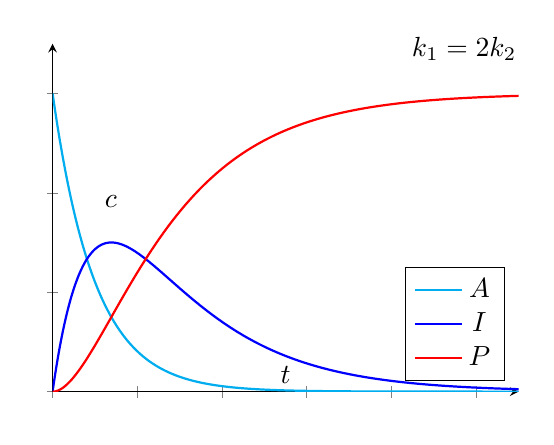
\begin{tikzpicture}
    \begin{axis}[
        title = {$k_1=2k_2$},
        title style={at={(0.75,1)},anchor=north west},
        width = 7.5cm,
        height = 6cm,
        legend pos = south east,
        x label style={at={(axis description cs:0.5,0.1)},anchor=north},
        y label style={at={(axis description cs:0.125,0.5)},rotate=270,anchor=south},
        xlabel = {$t$},
        ylabel = {$c$},
        axis lines = left,
        ymax = 3.5,
        domain = 0:5.5,
        samples = 400,
        xticklabels={},
        yticklabels={}
    ]
    \addplot [thick, cyan] {3*e^(-2*x)};
    \addplot [thick, blue] {3*2*(e^(-x)-e^(-2*x))};
    \addplot [thick, red] {3*(1-(2*e^(-x)-e^(-2*x)))};
    \legend {$\con{A}$,$\con{I}$,$\con{P}$}
    \end{axis}
\end{tikzpicture}
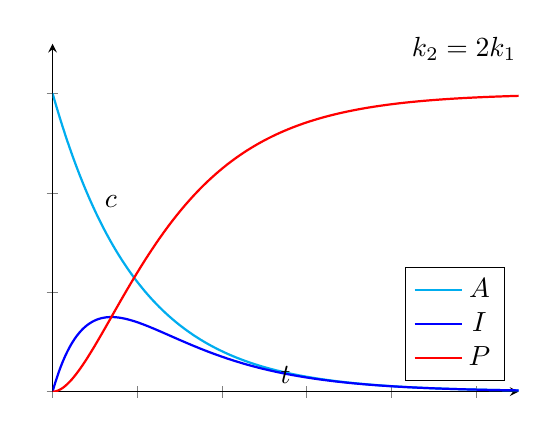
\begin{tikzpicture}
    \begin{axis}[
        title = {$k_2=2k_1$},
        title style={at={(0.75,1)},anchor=north west},
        width = 7.5cm,
        height = 6cm,
        legend pos = south east,
        x label style={at={(axis description cs:0.5,0.1)},anchor=north},
        y label style={at={(axis description cs:0.125,0.5)},rotate=270,anchor=south},
        xlabel = {$t$},
        ylabel = {$c$},
        axis lines = left,
        ymax = 3.5,
        domain = 0:5.5,
        samples = 400,
        xticklabels={},
        yticklabels={}
    ]
    \addplot [thick, cyan] {3*e^(-x)};
    \addplot [thick, blue] {3*(e^(-x)-e^(-2*x))};
    \addplot [thick, red] {3*(1-(2*e^(-x)-e^(-2*x)))};
    \legend {$\con{A}$,$\con{I}$,$\con{P}$}
    \end{axis}
\end{tikzpicture}
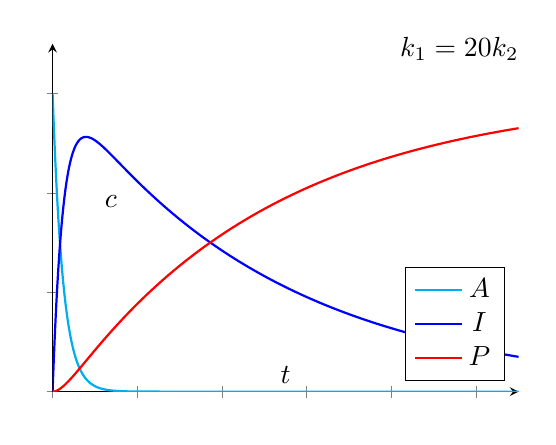
\begin{tikzpicture}
    \begin{axis}[
        title = {$k_1=20k_2$},
        title style={at={(0.725,1)},anchor=north west},
        width = 7.5cm,
        height = 6cm,
        legend pos = south east,
        x label style={at={(axis description cs:0.5,0.1)},anchor=north},
        y label style={at={(axis description cs:0.125,0.5)},rotate=270,anchor=south},
        xlabel = {$t$},
        ylabel = {$c$},
        axis lines = left,
        ymax = 3.5,
        domain = 0:5.5,
        samples = 400,
        xticklabels={},
        yticklabels={}
    ]
    \addplot [thick, cyan] {3*e^(-8*x)};
    \addplot [thick, blue] {3/7.6*8*(e^(-0.4*x)-e^(-8*x))};
    \addplot [thick, red] {3*(1+(0.4*e^(-8*x)-8*e^(-0.4*x))/7.6)};
    \legend {$\con{A}$,$\con{I}$,$\con{P}$}
    \end{axis}
\end{tikzpicture}
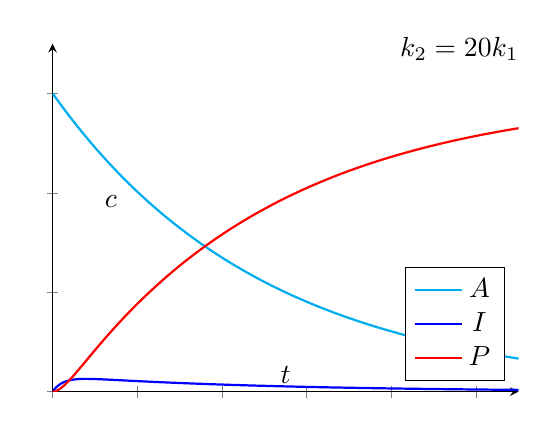
\begin{tikzpicture}
    \begin{axis}[
        title = {$k_2=20k_1$},
        title style={at={(0.725,1)},anchor=north west},
        width = 7.5cm,
        height = 6cm,
        legend pos = south east,
        x label style={at={(axis description cs:0.5,0.1)},anchor=north},
        y label style={at={(axis description cs:0.125,0.5)},rotate=270,anchor=south},
        xlabel = {$t$},
        ylabel = {$c$},
        axis lines = left,
        ymax = 3.5,
        domain = 0:5.5,
        samples = 400,
        xticklabels={},
        yticklabels={}
    ]
    \addplot [thick, cyan] {3*e^(-0.4*x)};
    \addplot [thick, blue] {3/7.6*0.4*(e^(-0.4*x)-e^(-8*x))};
    \addplot [thick, red] {3*(1+(0.4*e^(-8*x)-8*e^(-0.4*x))/7.6)};
    \legend {$\con{A}$,$\con{I}$,$\con{P}$}
    \end{axis}
\end{tikzpicture}
\end{document}
\end{figure}
当$k_1>k_2$时,可以发现反应\ce{A}迅速消耗,同时生成了一定量的中间体\ce{I},再转化为产物\ce{P}.%
而当$k_2\gg k_1$时,可以看到在相当长的一段时间里,$\con{I}$的浓度变化不大(并且相当的低),%
我们可以从前面的结果对这一猜测进行证明.
\begin{derivation}
    首先,直观地来说,如果$k_2\gg k_1$,这说明第二步反应的速率相对于第一步反应更快.因此,在反应进行不久后,%
    我们可以认为一定时间内\ce{A}转化为\ce{I}后立即转化为\ce{P}.在这段时间内,$\con{I}$随时间变化不大,%
    即$\dfrac{\di\con{I}}{\di t}\sim0$,于是
    \[k_2\con{I}=k_1\con{A}\]
    于是
    \[\con{I}=\dfrac{k_1}{k_2}\con{A}\]
    这表明$\con{I}$与$\con{A}$成正比例关系,比例系数为$\dfrac{k_1}{k_2}$.\\
    现在从定量的角度说明这一结果.我们有
    \[\dfrac{\con{I}}{\con{A}}=\dfrac{k_1}{k_2-k_1}\left(1-\e^{\left(k_1-k_2\right)t}\right)\]
    如果$k_2\gg k_1$,那么$k_1-k_2\ll0$.于是$1-\e^{\left(k_1-k_2\right)t}\sim1$.又
    \[\dfrac{k_1}{k_2-k_1}\sim\dfrac{k_1}{k_2}\]
    从而
    \[\dfrac{\con{I}}{\con{A}}=\dfrac{k_1}{k_2}\]
    尽管在作此近似后,$\con{I}$随$\con{A}$变化而变化,但由于比例系数$\dfrac{k_1}{k_2}$很小,因此我们的假设$\dfrac{\di\con{I}}{\di t}\sim0$仍然是成立的.%
    由此,我们可以得到
    \[\dfrac{\di\con{P}}{\di t}=k_2\con{I}=k_1\con{A}\]
    这一式子与\ce{A}直接生成\ce{P}的积分速率方程相同.%
    在\tbf{7C.2.1}令$k_2\gg k_1$,亦可以得到相同的结果.
\end{derivation}
这就是在动力学中非常重要的\tbf{稳态近似}.
\begin{theorem}[7C.2.2 稳态近似]
    连续反应中的不稳定中间体的净生成速率可以近似视作$0$.%
    在经历反应的\tbf{诱导期}(即中间体\ce{I}在反应初始时的生成)后,在反应的主要阶段,其浓度变化都很小.
\end{theorem}
需要说明的是,这里的“浓度变化很小”并不指的是$\con{I}$不变,而是$\dfrac{\di\con{I}}{\di t}$视作$0$.%
尽管这两个说法看起来有点矛盾,不过我们始终应当将目光放在产物和反应物等主要物质上,因此主要是通过稳态近似得出联系几种物质的等量关系,%
而非关注中间体本身的浓度.\\
\indent 前面推导中的\ce{I}就是不稳定中间体,它被消耗的速率常数$k_2$远大于生成的速率常数$k_1$,%
因而相对的难以生成而容易消耗.我们将在\tbf{7E}中讲述速率常数与活化能的关系,%
进而说明满足这样条件的中间体\ce{I}的能量相对而言比较高.\\
\indent 我们所说的不稳定中间体,一般而言可以根据你的化学知识储备判断,比如各种自由基和不稳定的分子等等.\\
\indent 应用稳态近似,我们可以将体系中所有不稳定中间体所对应的微分方程变为一个确定的等量关系,从而大大简化计算.%
我们将在本节之后的例子和本章的习题中反复应用这一重要定律.\vspace{4pt}\\
\Part{速率控制步骤}
\indent 尽管本小节放在\tbf{7E}介绍似乎更为合适,但我们仍然可以从连续反应的积分速率方程中得出一些有用的结论.%
前面我们已经知道,当$k_2\gg k_1$时,利用稳态近似可得
\[\dfrac{\di\con{P}}{\di t}=-\dfrac{\di\con{A}}{\di t}\]
即\ce{A}消耗的速率与\ce{P}生成的速率相等.这表明反应的速率大体上由第一步的速率决定.
\begin{hint}
    认识到在稳态近似后\ce{A -> I}和\ce{I -> P}的速率相同是十分重要的:与\ce{A}相比,%
    \ce{I}的浓度是如此之低,以至于尽管$k_2\gg k_1$,这两步反应的速率仍然几乎相同.\\
    因此,通常所说的“第一步慢,第二步快,所以第一步是决速步”是有问题的.实际上是两个反应速率相同,而速率常数有差别.
\end{hint}
而当$k_1\gg k_2$时,在相当短的一段时间内,\ce{A}就被消耗完全,而体系中仍然剩余大量的\ce{I}.%
此时,就可以视作\ce{I}向\ce{P}转化的反应.因此,此时反应的速率大体上由第二步的速率决定.
\begin{definition}[7C.2.3 速率控制步骤]
    连续反应中最慢的步骤称为反应的\tbf{速率控制步骤}(又称为\tbf{决速步}).%
    通常而言,反应的速率由决速步的速率决定.
\end{definition}
这便是我们避免繁杂的微分方程而得出的第二个经验结论.%
这里的最慢并非实际速率,而是被速率常数所决定的.\vspace{4pt}\\
\Part{平衡态假设}
\indent 现在,让我们考虑一个稍加复杂些的体系,即反应物\ce{A}与中间体\ce{I}之间存在不可忽略的平衡.
\begin{derivation}
    考虑连续反应
    \begin{tightcenter}
        \ce{A <=>T[$k_1$][$k_{-1}$] I ->T[$k_2$] P}
    \end{tightcenter}
    我们假定系统仍然满足稳态近似的条件,即$k_1\gg k_2$.这样就有
    \[\dfrac{\di\con{I}}{\di t}=k_1\con{A}-\left(k_{-1}+k_2\right)\con{I}=0\]
    于是
    \[\con{I}=\dfrac{k_1}{k_{-1}+k_2}\con{A}\]
    如果逆反应的速率常数远小于第二步反应,这就是前面提到的稳态近似.%
    而如果这一关系恰好相反,即$k_{-1}\gg k_2$,就有
    \[\con{I}=\dfrac{k_1}{k_{-1}}\con{A}\]
    我们知道第一步平衡时$k_{-1}\con{I}=k_1\con{A}$,即$K_1=\dfrac{\con I}{\con A}=\dfrac{k_1}{k_{-1}}$,%
    这恰好是第一步反应处于平衡时需要满足的关系式.\\
    这和我们做的近似是一致的,即达成平衡的速率相对于\ce{I}被消耗的速率总是很快,%
    以至于在反应进行的大部分时间里我们都可以认为\ce{A}与\ce{I}处于平衡中.这样,反应的速率方程即为
    \[\dfrac{\di\con{P}}{\di t}=k_2\con{I}=\dfrac{k_1k_2}{k_{-1}}\con{A}=K_1k_2\con{A}\]

\end{derivation}
\begin{theorem}[7C.2.4 平衡态假设]
    在速率控制步骤前的对峙反应可以近似地认为处于平衡态.
\end{theorem}
大部分时候,用到平衡态假设的步骤都会特意标注反应是\tbf{快速平衡},或者只有平衡常数$K$而没有正逆反应的速率常数.%
在不能明确判断平衡的正逆反应的速率时,需要谨慎使用平衡态假设.\\
\indent 平衡态假设事实上是稳态近似的进一步推论.如果中间体的转化和前一步平衡的速率常数差别不大,%
那么我们仍有$\con{I}=\dfrac{k_1}{k_{-1}+k_2}\con{A}$这一关系,其中的每一项都不能忽略.
\end{document}
\newpage\documentclass{ctexart}
\usepackage{PhysicalChemistryNote}

\begin{document}\pagestyle{plain}
\noindent\tbf{\LARGE 7D 反应机理示例}\vspace{15pt}\\
\indent 在这一节中,我们将综合运用你的数学与化学知识来推导各种反应的速率方程,%
并加深你对\tbf{7C}中学习的理论知识的印象与实用的技巧.\vspace{12pt}\\
\Section{7D.1 链反应}
\Part{链反应的基本概念}
\indent 在化学动力学中有一类特殊的反应,只需用热,光或辐射等方法使反应引发,%
体系就能通过活性组分(通常是自由基或原子)相继发生一系列的连续反应,%
像链条一样自动地发展下去.
\begin{definition}[7D.1.1 链反应]
    \tbf{链反应}(又称\tbf{连锁反应}),是指反应的产物或副产物又可作为其他反应的原料,%
    从而使反应反复发生.在化学中,链反应通常在光,热,辐射或引发剂作用下,反应中交替产生活性中间体(如自由原子或自由基),%
    从而使反应一直进行下去.
\end{definition}
按照活性物质数量的变化,链反应主要有三个过程.
\begin{definition}[7D.1.2 链反应的过程]
    在链反应中,产生活性中间体的过程称为\tbf{链引发},%
    活性中间体与反应物分子反复作用生成产物的过程称为\tbf{链增长}或\tbf{链传递},%
    活性中间体最后湮灭的过程称为\tbf{链终止}.
\end{definition}
一般的链增长过程中,一个活性中间体产生一个新的活性中间体.例如\ce{Cl.}与\ce{H2}的反应:
\begin{tightcenter}
    \ce{Cl. + H2 -> HCl + H.}
\end{tightcenter}
不过,在部分链增长过程中,一个活性中间体也可能产生数个活性中间体.例如\ce{H.}与\ce{O2}的反应:
\begin{tightcenter}
    \ce{H. + O2 -> HO. + O.}
\end{tightcenter}
据此,我们可以按照链增长的性质对链反应进行分类.
\begin{definition}[7D.1.3 直链反应与支链反应]
    一个活性中间体只能产生一个新的活性中间体的反应称为\tbf{直链反应},%
    可以产生两个或多个新的活性中间体的反应称为\tbf{支链反应}.
\end{definition}
我们将在接下来对这些链反应的速率方程进行详细地讨论.\vspace{4pt}\\
\Part{直链反应——\ce{H2}与卤素单质的自由基反应}
\indent 对中间体的研究表明,\ce{H2}与\ce{X2}(其中$\ce{X}=\ce{Cl},\ce{Br},\ce{I}$)在光照或加热下的化合反应%
的机理是不同的.我们先从最简单的\ce{H2}与\ce{Cl2}的反应开始.
\begin{derivation}\setcounter{equation}{0}
    \ce{H2}与\ce{Cl2}通过自由基反应生成\ce{HCl}的反应机理如下.
    \begin{tightcenter}
        \ce{Cl2 <=>T[$k_1$][$k_{-1}$] 2Cl.}\\
        \ce{Cl. + H2 ->T[$k_2$] HCl + H.}\\
        \ce{H. + Cl2 ->T[$k_3$] HCl + Cl.}
    \end{tightcenter}
    由于产物\ce{HCl}十分稳定,因此忽略后两个反应的逆反应.\\
    体系中的不稳定中间体为\ce{H.}与\ce{Cl.},分别对它们稳态近似有
    \begin{equation}
        \dfrac{\di\con{H.}}{\di t}=k_2\con{Cl.}\con{H2}-k_3\con{H.}\con{Cl2}=0
    \end{equation}
    \begin{equation}
        \dfrac{\di\con{Cl.}}{\di t}=2k_1\con{Cl2}-2k_{-1}\con{Cl.}^2-k_2\con{Cl.}\con{H2}+k_3\con{H.}\con{Cl2}=0
    \end{equation}
    将(2)减去(1)可得
    \begin{equation}
        2k_1\con{Cl2}-2k_{-1}\con{Cl.}^2=0
    \end{equation}
    于是
    \begin{equation}
        \con{Cl.}=\sqrt{\dfrac{k_1}{k_{-1}}\con{Cl2}}
    \end{equation}
    由(1)可得
    \begin{equation}
        \dfrac{\di\con{HCl}}{\di t}=k_2\con{Cl.}\con{H2}+k_3\con{H.}\con{Cl2}=2k_2\con{Cl.}\con{H2}
    \end{equation}
    将(4)代入(5)可得
    \begin{equation}
        \dfrac{\di\con{HCl}}{\di t}=2k_2\con{Cl.}\con{H2}=2k_2\sqrt{\dfrac{k_1}{k_{-1}}}\con{H2}\con{Cl2}^{\frac12}
    \end{equation}
    因此反应对\ce{H2}为一级,对\ce{Cl2}为二分之一级.
\end{derivation}

\end{document}
\newpage\documentclass{ctexart}
\usepackage{PhysicalChemistryNote}

\begin{document}\pagestyle{plain}
\noindent\tbf{\LARGE 7E 温度对反应速率的影响}\vspace{15pt}\\
\indent 实验表明,大多数化学反应的速率总是随着温度升高而增加.我们将从理论上对此给出解释,%
并说明速率常数与温度满足的关系.在本节的最后,我们也将介绍一种测定速率常数的重要办法.\vspace{12pt}
\Section{7E.1 Arrhenius方程}

\end{document}
\newpage\documentclass{ctexart}
\usepackage{PhysicalChemistryNote}

\begin{document}\pagestyle{plain}
\noindent\tbf{\LARGE Ex7 习题}\vspace{15pt}\\
\indent 我们将在本章的习题中给出更多的例题以供你巩固动力学知识.
\setcounter{Pcounter}{0}
\stepcounter{Pcounter}
\begin{problem}[P.7.\arabic{Pcounter}]
    Heck偶联反应为代表的过渡金属催化的偶联反应.这一反应的通式如下.
    \begin{tightcenter}
        \ce{ArBr + RCH=CH2 ->T[Pd catalyst][AcONa] ArCH=CHR + AcOH + NaBr}
    \end{tightcenter}
    这一反应的机理可以简化如下.
    \begin{tightcenter}
        \ce{E + A <=>T[$k_1$][$k_{-1}$] EA} \\
        \ce{EA + B ->T[$k_2$] E + P}
    \end{tightcenter}
    其中\ce{E}为\ce{Pd}催化剂,\ce{A}为溴代物,\ce{B}为原料烯烃,\ce{P}为产物烯烃.
    \begin{enumerate}[label=\tbf{\arabic{Pcounter}-\arabic*},topsep=0pt,parsep=0pt,itemsep=0pt,partopsep=0pt]
        \item 推导总反应速率$r$(以生成产物\ce{P}的速率记)的表达式.
        \item 记$\con{ex}=\con{B}_0-\con{A}_0$为两种底物的起始浓度之差,$\con{E}_0$为催化剂的总浓度.试证明反应速率$r$可以写成如下形式
            \[r=a\dfrac{\con{ex}\con{A}+\con{A}^2}{1+b\con{A}}\con{E}_0\]
            并求出系数$a,b$的表达式.
    \end{enumerate}
\end{problem}
\begin{solution}
    \begin{enumerate}[label=\tbf{\arabic{Pcounter}-\arabic*},topsep=0pt,parsep=0pt,itemsep=0pt,partopsep=0pt]
        \item 这事实上不过是米氏方程的变形.我们对\ce{EA}稳态近似可得
            \[\dfrac{\di\con{EA}}{\di t}=k_1\con{E}\con{A}-k_{-1}\con{EA}-k_2\con{EA}\con{B}=0\]
            于是
            \[\con{EA}=\dfrac{k_1\con{E}\con{A}}{k_{-1}+k_2\con{B}}\]
            由物料守恒$\con{E}+\con{EA}=\con{E}_0$可得
            \[\con{EA}\left(1+\dfrac{k_{-1}+k_2\con{B}}{k_1\con{A}}\right)=\con{E}_0\]
            于是
            \[r=k_2\con{EA}\con{B}=\dfrac{k_1k_2\con{E}_0\con{A}\con{B}}{k_{-1}+k_1\con{A}+k_2\con{B}}\]
        \item 根据计量数有$\con{ex}=\con{B}_0-\con{A}_0=\con{B}-\con{A}$.代入第一问的结果可得
            \[r=\dfrac{k_1k_2\con{E}_0\con{A}\left(\con{A}+\con{ex}\right)}{k_{-1}+k_1\con{A}+k_2\left(\con{A}+\con{ex}\right)}
            =\dfrac{k_1k_2}{k_{-1}+k_2\con{ex}}\cdot\dfrac{\con{ex}\con{A}+\con{A}^2}{1+\dfrac{k_1+k_2}{k_{-1}+k_2\con{ex}}\con{A}}\con{E}_0\]
            于是有
            \[a=\dfrac{k_1k_2}{k_{-1}+k_2\con{ex}}\ \ \ \ \ b=\dfrac{k_1+k_2}{k_{-1}+k_2\con{ex}}\]
            这样,由于$\con{ex}$和$\con{E}_0$都是已知的量,我们就可以通过测定$\con{A}$得出反应速率$r$.
    \end{enumerate}
\end{solution}
\stepcounter{Pcounter}
\begin{problem}[P.7.\arabic{Pcounter}]
    铁卟啉(\ce{FeP})是细胞色素(P-450)的活性中心,具有将各种氧供体的氧原子活化并转移至底物的能力.%
    研究人员为模拟活体内的加氧酶催化$\beta$-胡萝卜素(\ce{$\beta$})分解为维生素\ce{A}(\ce{VA})的反应,%
    以\ce{FeP}为催化剂,间氯过氧化苯甲酸(\ce{CPBA})为氧化剂,研究了$\beta$-胡萝卜素的分解反应动力学.%
    研究中\ce{FeP}和\ce{CPBA}的浓度可视为不变.无论是否存在催化剂\ce{FeP},该分解反应对$\beta$-胡萝卜素均为一级反应.\\
    \tbf{实验A}.在无\ce{FeP}的情况下,$\beta$-胡萝卜素-间氯过氧化苯甲酸反应体系($\beta-\ce{CPBA}$)的反应机理$1$如下%
    (其中$\beta\ast\ce{CPBA}$为反应中间物,\ce{CBA}为间氯苯甲酸):
    \begin{tightcenter}
        \ce{$\beta$ + CPBA <=>T[$K_i'$] $\beta\ast\ce{CPBA}$}\\
        \ce{$\beta\ast\ce{CPBA}$ ->T[$k_2'$] VA + CBA}
    \end{tightcenter}
    \tbf{实验B}.以\ce{FeP}为催化剂,$\beta$-胡萝卜素-间氯过氧化苯甲酸-铁卟啉反应体系($\beta-\ce{CPBA}-\ce{FeP}$)的反应机理$2$如下%
    (其中$\ce{FeOP}\ast\ce{CBA},\beta\ast\ce{FeOP}\ast\ce{CBA},\beta\ast\ce{CPBA}$为反应中间物):
    \begin{tightcenter}
        \ce{FeP + CPBA <=>T[$K_1$] $\ce{FeOP}\ast\ce{CBA}$}\\
        \ce{$\ce{FeOP}\ast\ce{CBA}$ + $\beta$ <=>T[$K_2$] $\beta\ast\ce{FeOP}\ast\ce{CBA}$}\\
        \ce{$\beta\ast\ce{FeOP}\ast\ce{CBA}$ ->T[$k_1$] VA + FeP + CBA}\\
        \ce{$\beta$ + CPBA <=>T[$K_i$] $\beta\ast\ce{CPBA}$}\\
        \ce{$\beta\ast\ce{CPBA}$ ->T[$k_2$] VA + CBA}
    \end{tightcenter}
    对该体系的实验结果进行曲线拟合,可得以下数据(其中$k_{\text{obs}}$为反应的表观速率常数).
    \vspace{-5pt}\begin{table}[H]\centering
        \begin{tabular}{|c|c|c|c|}
            \hline
                $T/\text{K}$ & $k_1/\text{s}^{-1}$ & $k_2/\text{s}^{-1}$ & $k_{\text{obs}}/\text{s}^{-1}$ \\ \hline
                $293.2$ & $4.869\times10^{-3}$ & $1.350\times10^{-4}$ & $5.865\times10^{-4}$ \\ \hline
                $301.2$ & $7.731\times10^{-3}$ & $2.398\times10^{-4}$ & $9.795\times10^{-4}$ \\ \hline
        \end{tabular}
    \end{table}\vspace{-15pt}
    \begin{enumerate}[label=\tbf{\arabic{Pcounter}-\arabic*},topsep=0pt,parsep=0pt,itemsep=0pt,partopsep=0pt]
        \item 对$\beta-\ce{CPBA}$体系,测得
            \[k_{\text{obs}}'(293.2\K)=4.795\times10^{-4}\text{ s}^{-1}\ \ \ \ \ k_{\text{obs}}'(301.2\K)=8.285\times10^{-4}\text{ s}^{-1}\]
            求反应的表观活化能$E_{a,\text{obs}}'$.
        \item 根据反应机理$2$,推导$\beta\ast\ce{CPBA}\ast\ce{FeP}$体系中$-\dfrac{\di[\beta]}{\di t}$与$[\beta]$间关系的速率方程,并给出$k_{\text{obs}}$的表达式.
        \item 已知$\beta\ast\ce{CPBA}\ast\ce{FeP}$体系反应的表观活化能$E_{\text{obs}}=47.07\kJm$和机理$2$中第三步的活化能$E_{a,1}=42.43\kJm$,计算机理$2$中第五步的活化能$E_{a,2}$.
        \item 分别根据以下条件,说明$\beta-\ce{CPBA}$和$\beta\ast\ce{CPBA}\ast\ce{FeP}$中哪一个体系的反应更有利.
            \begin{enumerate}[label=\tbf{\arabic{Pcounter}-4-\arabic*},topsep=0pt,parsep=0pt,itemsep=0pt,partopsep=0pt,leftmargin=10pt]
                \item $E_{a,1}$与$E_{a,2}$的结果.
                \item $E_{a,\text{obs}}$与$E_{a,\text{obs}}'$的结果.
            \end{enumerate}
    \end{enumerate}
\end{problem}
\begin{solution}
    \begin{enumerate}[label=\tbf{\arabic{Pcounter}-\arabic*},topsep=0pt,parsep=0pt,itemsep=0pt,partopsep=0pt]
        \item 根据Arrhenius方程有
            \[\ln\dfrac{k_{\text{obs}}'\left(T_1\right)}{k_{\text{obs}}'\left(T_2\right)}=\dfrac{E_{a,\text{obs}}'}{R}\left(\dfrac{1}{T_2}-\dfrac{1}{T_1}\right)\]
            代入题中数据可得
            \[\ln\dfrac{4.795\times10^{-4}}{8.285\times10^{-4}}=\dfrac{E_{a,\text{obs}}'}{8.314\JmK}\left(\dfrac{1}{293.2\K}-\dfrac{1}{301.2\K}\right)\]
            解得
            \[E_{a,\text{obs}}=50.19\kJm\]
        \item 我们在\tbf{7D}的酶促反应的示例中大多是推导产物的生成速率,而这道题则有些不同.我们要求反应物$\beta$的消耗速率$-\dfrac{\di[\beta]}{\di t}$.%
            并且,由于题目中已经说明酶\ce{FeP}的浓度可视为不变,因此我们并不能使用一般的酶的物料守恒求解.\\
            我们遇到的最大的困难在于有关$\beta$的反应全部出现在快速平衡中,而题目并未给出快速平衡的速率常数,这使得我们无法直接写出$-\dfrac{\di[\beta]}{\di t}$的显式表达式.\\
            因此,我们需要采取一些间接的方法.如果我们用另一物质的浓度表示$[\beta]$,然后将这一表达式对时间$t$求导,即可用这一物质的消耗或生成速率表达$-\dfrac{\di[\beta]}{\di t}$.\\
            由于这一体系的净反应为\ce{$\beta$ + CPBA -> VA + CBA},因此$\beta$的物料守恒为
            \[[\beta]_0=\con{VA}+[\beta]+[\beta\ast\ce{FeOP}\ast\ce{CBA}]+[\beta\ast\ce{CBA}]\]
            直接对此式求导仍然是不可行的,因为后两个中间体的浓度也会随着$[\beta]$的变化而变化.我们需要写出这一关系.%
            根据平衡态假设可知
            \[[\beta\ast\ce{FeOP}\ast\ce{CBA}]=K_1K_2\con{FeP}\con{CPBA}[\beta]\]
            \[[\beta\ast\ce{CBA}]=K_i\con{CPBA}[\beta]\]
            代入上述物料守恒可得
            \[[\beta]_0=\con{VA}+\left(1+K_1K_2\con{FeP}\con{CPBA}+K_i\con{CPBA}\right)[\beta]\]
            我们将上式对时间$t$求导可得
            \[-\dfrac{\di[\beta]}{\di t}=\dfrac{1}{1+K_1K_2\con{FeP}\con{CPBA}+K_i\con{CPBA}}\dfrac{\di\con{VA}}{\di t}\]
            又因为
            \[\begin{aligned}
                \dfrac{\di\con{VA}}{\di t}
                &= k_1[\beta\ast\ce{FeOP}\ast\ce{CBA}]+k_2[\beta\ast\ce{CBA}] \\
                &= \left(k_1K_1K_2\con{FeP}\con{CPBA}+k_2K_i\con{CPBA}\right)[\beta]
            \end{aligned}\]
            于是
            \[-\dfrac{\di[\beta]}{\di t}=\dfrac{k_1K_1K_2\con{FeP}\con{CPBA}+k_2K_i\con{CPBA}}{1+K_1K_2\con{FeP}\con{CPBA}+K_i\con{CPBA}}[\beta]\]
            于是
            \[k_{\text{obs}}=\dfrac{\left(k_1K_1K_2\con{FeP}+k_2K_i\right)\con{CPBA}}{1+\left(K_1K_2\con{FeP}+K_i\right)\con{CPBA}}\]
            如果你认为一个$\beta$可以变成一个\ce{VA},从而认为$-\dfrac{\di[\beta]}{\di t}=\dfrac{\con{VA}}{\di t}$,那就大错特错了.这道题最重要的地方就在于%
            中间体的浓度也会随时间而变化,并且其浓度都与$[\beta]$成正比关系,因此需要统一代入.
        \item 这一小问的做法与\tbf{\arabic{Pcounter}-1}是完全一致的,我们代入数据即可得
            \[\ln\dfrac{1.350\times10^{-4}}{2.398\times10^{-4}}=\dfrac{E_{a,2}}{8.314\JmK}\left(\dfrac{1}{293.2\K}-\dfrac{1}{301.2\K}\right)\]
            解得
            \[E_{a,2}=52.73\kJm\]
        \item 这一小问要求我们从两个角度分析\ce{FeP}对$\beta$氧化为\ce{VA}的反应是否有利.比较两个不同的反应机理,%
            既可以从具体决速步的活化能判断,也可以从有无催化剂时反应的表观活化能判断.
            \begin{enumerate}[label=\tbf{\arabic{Pcounter}-4-\arabic*},topsep=0pt,parsep=0pt,itemsep=0pt,partopsep=0pt,leftmargin=10pt]
                \item 从反应机理来看,机理$1$的步骤与机理$2$的后两步完全相同,这意味着这两个反应的速率常数和活化能相同(我们的计算确实支持这一点).%
                    但对于机理$2$有$E_{a,1}<E_{a,2}$,这意味着反应可以经过一个活化能更小的步骤进行,因此\ce{FeP}对这一反应是有利的.
                \item 从表观活化能来看有$E_{a,\text{obs}}<E_{a,\text{obs}}'$,这意味着通过机理$2$进行的反应的总体的活化能更小,这也可以得出\ce{FeP}对这一反应是有利的.
            \end{enumerate}
    \end{enumerate}
\end{solution}
\stepcounter{Pcounter}
\begin{problem}[P.7.\arabic{Pcounter} 岩石变化动力学]
    斜方辉石\ce{[(Mg,Fe)2Si2O6]}是地壳和上地幔的主要组成矿物之一,在其晶体结构中包含有两种不同的硅氧四面体\ce{(SiO3)2-}链,%
    分别称作\ce{A}链和\ce{B}链,基于这两种链的排布而形成了两种结构有差异的八面体空隙M1和M2,二者比例相同.%
    \ce{Mg^2+}和\ce{Fe^2+}便分布在这些八面体空隙中.由于M1和M2的空隙性质不同,%
    导致\ce{Mg^2+}和\ce{Fe^2+}对其占据的选择性不同,\ce{Fe^2+}倾向于占据M2位置.%
    一定条件下,两种离子可以发生不同位置的交换反应:
    \begin{tightcenter}
        \ce{Fe^2+({M1}) + Mg^2+({M2}) <=> Fe^2+({M2}) + Mg^2+({M1})}
    \end{tightcenter}
    为简便起见,\ce{Fe^2+({M1})},\ce{Mg^2+({M2})},\ce{Fe^2+({M2})}和\ce{Mg^2+({M1})}分别写作Fe(1),Fe(2),Mg(1)和Mg (2).%
    上述反应达平衡时,分配系数$K_D$为
    \[K_D=\dfrac{\chi_{\ce{Fe(2)}}\chi_{\ce{Mg(1)}}}{\chi_{\ce{Fe(1)}}\chi_{\ce{Mg(2)}}}\]
    其中,$\chi$为各离子占据相应位置的摩尔分数,例如:$\chi_{\ce{Fe(2)}}$为\ce{Fe^2+}离子占据M2位置的摩尔分数,其他同理.\\
    选择某一矿物样品,在$873\K$下进行处理,利用X射线衍射结合穆斯堡尔谱监测反应进行过程中上述物种占据不同位置情况随时间的变化,数据列入下表中.
    \vspace{-5pt}\begin{table}[H]\centering
        \begin{tabular}{|c|c|c|c|c|c|}
            \hline
                编号 & $t/\text{min}$ & $\chi_{\ce{Fe(1)}}$ & $\chi_{\ce{Mg(2)}}$ & $\chi_{\ce{Fe(2)}}$ & $\chi_{\ce{Mg(1)}}$ \\ \hline
                1   & 0     & 0.00450   & 0.9807    & 0.0174    & 0.9769 \\ \hline
                2	& 600   & 0.00420   & 0.9804    & 0.0176    & 0.9771 \\ \hline
                3	& 1920  & 0.00380   & 0.9801	& 0.0179	& 0.9774 \\ \hline
                4	& 3720	& 0.00361	& 0.9798	& 0.0183	& 0.9778 \\ \hline
                5	& 6000	& 0.00335	& 0.9795	& 0.0185	& 0.9780 \\ \hline
                6	& 11760	& 0.00281	& 0.9790	& 0.0191	& 0.9786 \\ \hline
                7	& 20300	& 0.00261	& 0.9788	& 0.0193	& 0.9788 \\ \hline
                8	& 29700	& 0.00233	& 0.9785	& 0.0195	& 0.9790 \\ \hline
                9	& 48165	& 0.00232	& 0.9785	& 0.0195	& 0.9790 \\ \hline
        \end{tabular}
    \end{table}\vspace{-15pt}
    \begin{enumerate}[label=\tbf{\arabic{Pcounter}-\arabic*},topsep=0pt,parsep=0pt,itemsep=0pt,partopsep=0pt]
        \item 计算分配系数$K_D$.(提示:合理判断并选择表中的数据.)
        \item 记上述反应的正,逆反应的速率常数分别为$k_1$和$k_{-1}$.假设正,逆反应速率表达形式均与基元反应类似,即反应速率分别与占据相应位置的各离子的摩尔分数$\chi$成正比.%
            据此,写出$K_D$与$k_1$和$k_{-1}$的关系式。
        \item 利用上表中起始阶段的数据(采用编号1到4的数据进行处理),计算$k_1$和$k_{-1}$的值.%
            (提示:可将\ce{Mg^2+}的摩尔分数视作常数,取0.9780.)
    \end{enumerate}
\end{problem}
\begin{solution}
    \begin{enumerate}[label=\tbf{\arabic{Pcounter}-\arabic*},topsep=0pt,parsep=0pt,itemsep=0pt,partopsep=0pt]
        \item 我们需要寻找平衡状态的数据以计算$K_D$.观察编号为8和9的数据,可以发现各物种的摩尔分数已经近似地不再变化,即达到平衡状态.%
            选取编号$9$的数据,可得
            \[K_D=\dfrac{\chi_{\ce{Fe(2)}}\chi_{\ce{Mg(1)}}}{\chi_{\ce{Fe(1)}}\chi_{\ce{Mg(2)}}}
            =\dfrac{0.9795\cdot0.0195}{0.9785\cdot0.00232}=8.41\]
            若选取编号$8$的数据得到$K_D=8.44$,亦可.
        \item 平衡时,正逆反应速率相等,即有
            \[k_1\chi_{\ce{Fe(2)}}\chi_{\ce{Mg(1)}}=k_{-1}\chi_{\ce{Fe(1)}}\chi_{\ce{Mg(2)}}\]
            又因为分配系数的定义为
            \[K_D=\dfrac{\chi_{\ce{Fe(2)}}\chi_{\ce{Mg(1)}}}{\chi_{\ce{Fe(1)}}\chi_{\ce{Mg(2)}}}\]
            结合上述两式可得
            \[K_D=\dfrac{k_1}{k_{-1}}\]
            事实上,这和一般的基元反应的平衡常数与正逆反应速率常数的关系是完全一致的.%
            在本题中,我们只不过不使用浓度,转而使用摩尔分数来表示反应速率.
        \item 为了求出摩尔分数随时间的关系,我们需要求出反应体系的积分速率方程.\\
            首先,体系的微分速率方程为
            \[\dfrac{\di\chi_{\ce{Fe(2)}}}{\di t}=-k_1\chi_{\ce{Fe(2)}}\chi_{\ce{Mg(1)}}+k_{-1}\chi_{\ce{Fe(1)}}\chi_{\ce{Mg(2)}}\]
            这一方程具有四个变量,难以进行进一步的积分运算,因此我们需要尽量减少和统一变量.%
            为此,首先将\ce{Mg^2+}的摩尔分数视作常数(不妨记作$\chi_{\ce{Mg}}$)后就有
            \[\dfrac{\di\chi_{\ce{Fe(2)}}}{\di t}=-k_1\chi_{\ce{Fe(2)}}\chi_{\ce{Mg}}+k_{-1}\chi_{\ce{Fe(1)}}\chi_{\ce{Mg}}
            =0.9780\left(-k_1\chi_{\ce{Fe(2)}}+k_{-1}\chi_{\ce{Fe(1)}}\right)\]
            随后,在\tbf{\arabic{Pcounter}-2}中我们知道$k_1$与$k_{-1}$的等量关系.将\tbf{\arabic{Pcounter}-1}中的$K_D$代入可得
            \[k_1=8.41 k_{-1}\]
            将此式代入速率方程可得
            \[\dfrac{\di\chi_{\ce{Fe(2)}}}{\di t}=0.9780k_{-1}\left(\chi_{\ce{Fe(1)}}-8.41\chi_{\ce{Fe(2)}}\right)\]
            现在我们来思考$\chi_{\ce{Fe(1)}}$和$\chi_{\ce{Fe(2)}}$的关系.体系中的\ce{Fe^2+}的总量是守恒的,即有
            \[n(\ce{Fe(1)})+n(\ce{Fe(2)})=n_0(\ce{Fe^2+})\]
            我们将两种空隙的数目,以及\ce{Fe^2+}占两种空隙的比例代入可得
            \[n(\ce{{M1}})\chi_{\ce{Fe(1)}}+n(\ce{{M2}})\chi_{\ce{Fe(2)}}=n_0(\ce{Fe^2+})\]
            由于题目中给出M1与M2的比例相同,因此有$n(\ce{{M1}})=n(\ce{{M2}})$.于是有
            \[\chi_{\ce{Fe(1)}}+\chi_{\ce{Fe(2)}}=\dfrac{n_0(\ce{Fe^2+})}{n(\ce{{M1}})}=2\chi_{\ce{Fe}}\]
            我们将$t=0$时的摩尔分数代入上式可得
            \[\chi_{\ce{Fe(1)}}+\chi_{\ce{Fe(2)}}=0.0219\]
            将这一等量关系代入速率方程以消去$\chi_{\ce{Fe(1)}}$,即可得到
            \[\dfrac{\di\chi_{\ce{Fe(2)}}}{\di t}=k_{-1}\left(\right)\]
    \end{enumerate}
\end{solution}
\end{document}
\end{document}